\begin{figure}[t]
  \centering
  \begin{subfigure}[b]{0.45\textwidth}
    \centering
    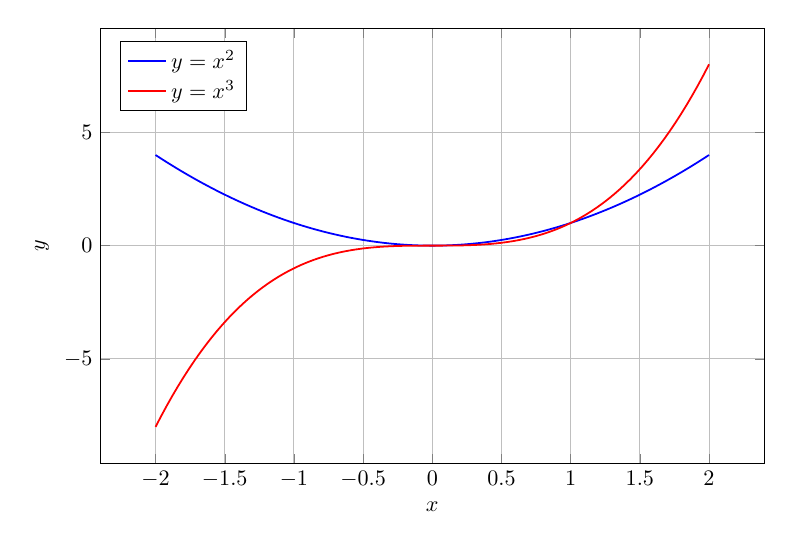
\begin{tikzpicture}[scale=0.8]
      \begin{axis}[
        xlabel={$x$},
        ylabel={$y$},
        grid=major,
        legend pos=north west,
        width=\textwidth,
        height=0.7\textwidth,
      ]
        \addplot[domain=-2:2, samples=100, blue, thick] {x^2};
        \addlegendentry{$y = x^2$}
        \addplot[domain=-2:2, samples=100, red, thick] {x^3};
        \addlegendentry{$y = x^3$}
      \end{axis}
    \end{tikzpicture}
    \caption{Polynomial functions}
    \label{fig:sample-a}
  \end{subfigure}
  \hfill
  \begin{subfigure}[b]{0.45\textwidth}
    \centering
    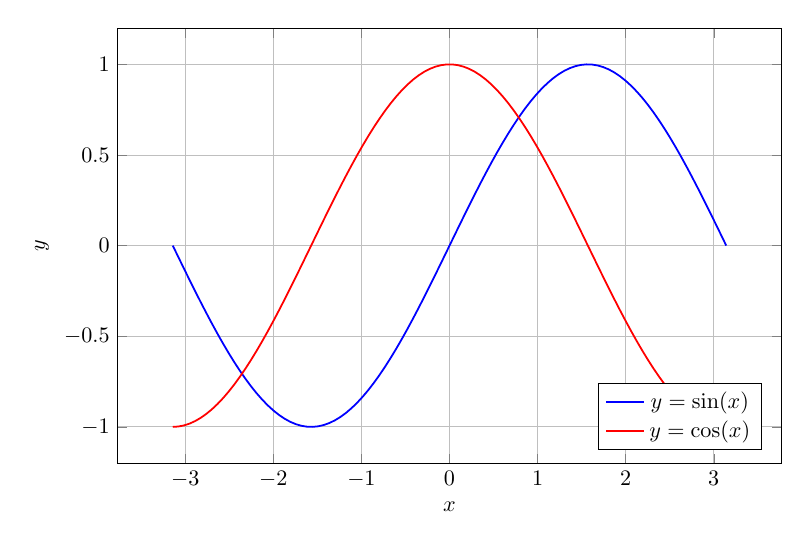
\begin{tikzpicture}[scale=0.8]
      \begin{axis}[
        xlabel={$x$},
        ylabel={$y$},
        grid=major,
        legend pos=south east,
        width=\textwidth,
        height=0.7\textwidth,
        domain=-pi:pi,
      ]
        \addplot[samples=100, blue, thick] {sin(deg(x))};
        \addlegendentry{$y = \sin(x)$}
        \addplot[samples=100, red, thick] {cos(deg(x))};
        \addlegendentry{$y = \cos(x)$}
      \end{axis}
    \end{tikzpicture}
    \caption{Trigonometric functions}
    \label{fig:sample-b}
  \end{subfigure}
  
  \vspace{0.5cm}
  
  \begin{subfigure}[b]{0.45\textwidth}
    \centering
    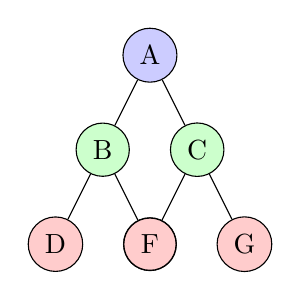
\begin{tikzpicture}[scale=0.8]
      % Tree structure
      \node[circle, draw, fill=blue!20] (root) at (0,0) {A}
        child {node[circle, draw, fill=green!20] {B}
          child {node[circle, draw, fill=red!20] {D}}
          child {node[circle, draw, fill=red!20] {E}}
        }
        child {node[circle, draw, fill=green!20] {C}
          child {node[circle, draw, fill=red!20] {F}}
          child {node[circle, draw, fill=red!20] {G}}
        };
    \end{tikzpicture}
    \caption{Binary tree structure}
    \label{fig:sample-c}
  \end{subfigure}
  \hfill
  \begin{subfigure}[b]{0.45\textwidth}
    \centering
    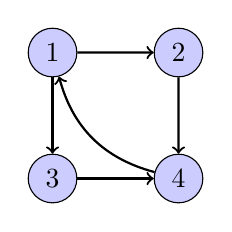
\begin{tikzpicture}[scale=0.8]
      % Directed graph
      \node[circle, draw, fill=blue!20] (1) at (0,2) {1};
      \node[circle, draw, fill=blue!20] (2) at (2,2) {2};
      \node[circle, draw, fill=blue!20] (3) at (0,0) {3};
      \node[circle, draw, fill=blue!20] (4) at (2,0) {4};
      
      \draw[->, thick] (1) -- (2);
      \draw[->, thick] (1) -- (3);
      \draw[->, thick] (2) -- (4);
      \draw[->, thick] (3) -- (4);
      \draw[->, thick, bend left] (4) to (1);
    \end{tikzpicture}
    \caption{Directed graph}
    \label{fig:sample-d}
  \end{subfigure}
  
  \caption{Examples of figures created with TikZ and PGFPlots. The package supports mathematical plots, tree structures, and graph visualizations.}
  \labelfig{sample}
\end{figure}
